\chapter{Repository, Terminal, and Computer-Use Agents}\label{ch:C23}
TestJack's October 2026 audit constructs prompt-grounded witness tests against candidates that passed existing coding evaluators; AgentHorizon separately examines computer-use evaluation with task instructions and execution trajectories~\cite{yao2026testjack,corpus261011050}. Both cases challenge the inference from a favorable grader response to completed work. They expose different observation gaps: a test suite may omit a stated requirement, while an interface snapshot may omit the action history needed to interpret the final state. Neither audit provides an infallible judge.

Coding agents operate on artifacts whose correctness is partly executable, but executable does not mean fully specified. A patch can satisfy the visible tests while violating a stated requirement that those tests omit, introducing a security regression, or modifying the tests themselves. An underspecified requirement instead needs adjudication before disagreement can refute the patch. Computer-use agents add another observation problem: a screenshot can show a plausible final state without proving that the requested object, recipient, or permission was selected. The shared objective is to connect task interpretation, environment interaction, and independently checkable evidence.

The central comparison is between complete configured systems. Model, harness, repository context, tool interface, execution environment, evaluator, and budget all influence results. Product names are insufficient experimental identifiers. This chapter analyzes these boundaries, gives concrete implementation and benchmark anchors, and distinguishes inspectable mechanisms from undocumented hosted behavior.

\section{Repository state as an executable environment}\label{sec:C23:repository}
A repository task is a partially observed transition problem. The agent observes selected files, search results, test outputs, and version-control metadata. It acts through edits, commands, dependency operations, and sometimes remote services. The true environment includes build tools, generated files, network dependencies, and hidden tests that may not appear in its initial context. Treating the task as text completion discards the execution feedback that makes repository-level work distinctive.

The action interface should preserve artifact identity. A patch request names its base revision and intended file changes; command execution records working directory, environment, exit status, and captured output. The test verdict binds to the resulting artifact digest. If the agent edits code after testing, the verdict must be invalidated or rerun. This mechanical correspondence is separate from whether the tests capture the intended behavior.

An execution attestation can make that boundary explicit. Let $A$ be the tested artifact, $D$ its declared dependency/environment manifest, and $e=(a,d,q,x,\tau)$ record their digests, the exact test invocation $q$, exit status $x$, and execution trace $\tau$. With $\kappa(\tau)=1$ denoting a complete, attributable invocation record, define
\begin{equation}
 v_e(A,D)=\mathbf1\{a=h(A)\}\mathbf1\{d=h(D)\}
          \mathbf1\{x=0\}\mathbf1\{\kappa(\tau)=1\}.
 \label{eq:C23:artifact_attestation}
\end{equation}
This predicate establishes provenance of a zero-exit execution for the declared inputs, assuming collision-resistant hashing and trustworthy records. It does not establish requirement coverage, authentic dependencies beyond the captured manifest, or absence of unrecorded network/environment changes. A failed command followed by a persuasive final message has $v_e=0$; an edit after testing changes $h(A)$ and invalidates the old attestation. Test discovery failures and a command that executes no relevant tests still require separate validation even when its exit status is zero.

The 2024 SWE-agent study established an influential interface baseline and demonstrates the importance of the agent-computer interface rather than model capability alone~\cite{yang2024sweagent}. Search, file navigation, editing, and error feedback change how effectively the model can act on repository state. The proper inference is interface sensitivity in the studied setting. It does not establish that one interface dominates across languages, repositories, models, and tool latency. A useful replication preserves the evaluator and workload while varying only the interaction surface.

The implementation anchor is an actual rollout through the published repository: model input construction, command interface, environment stepping, output truncation, and termination. A researcher should locate the callable that executes actions and the adapter that converts its results back into model-visible messages. Silent truncation or error normalization can materially change the policy. Comparing only prompt templates misses those mechanisms.

Repository isolation also matters. An agent should not see another benchmark task's generated artifacts or hidden test outcomes through a shared checkout or cache. The workspace, dependencies, and stateful tools need a reset policy. Reusing a build cache may be legitimate for cost analysis but must not transfer answer-bearing files across tasks. Separate a warm infrastructure cache from persistent semantic memory and report both explicitly.



Figure~\ref{fig:C23:overview} isolates the mechanism and its stated information boundaries.
\begin{figure}[!htbp]
\centering
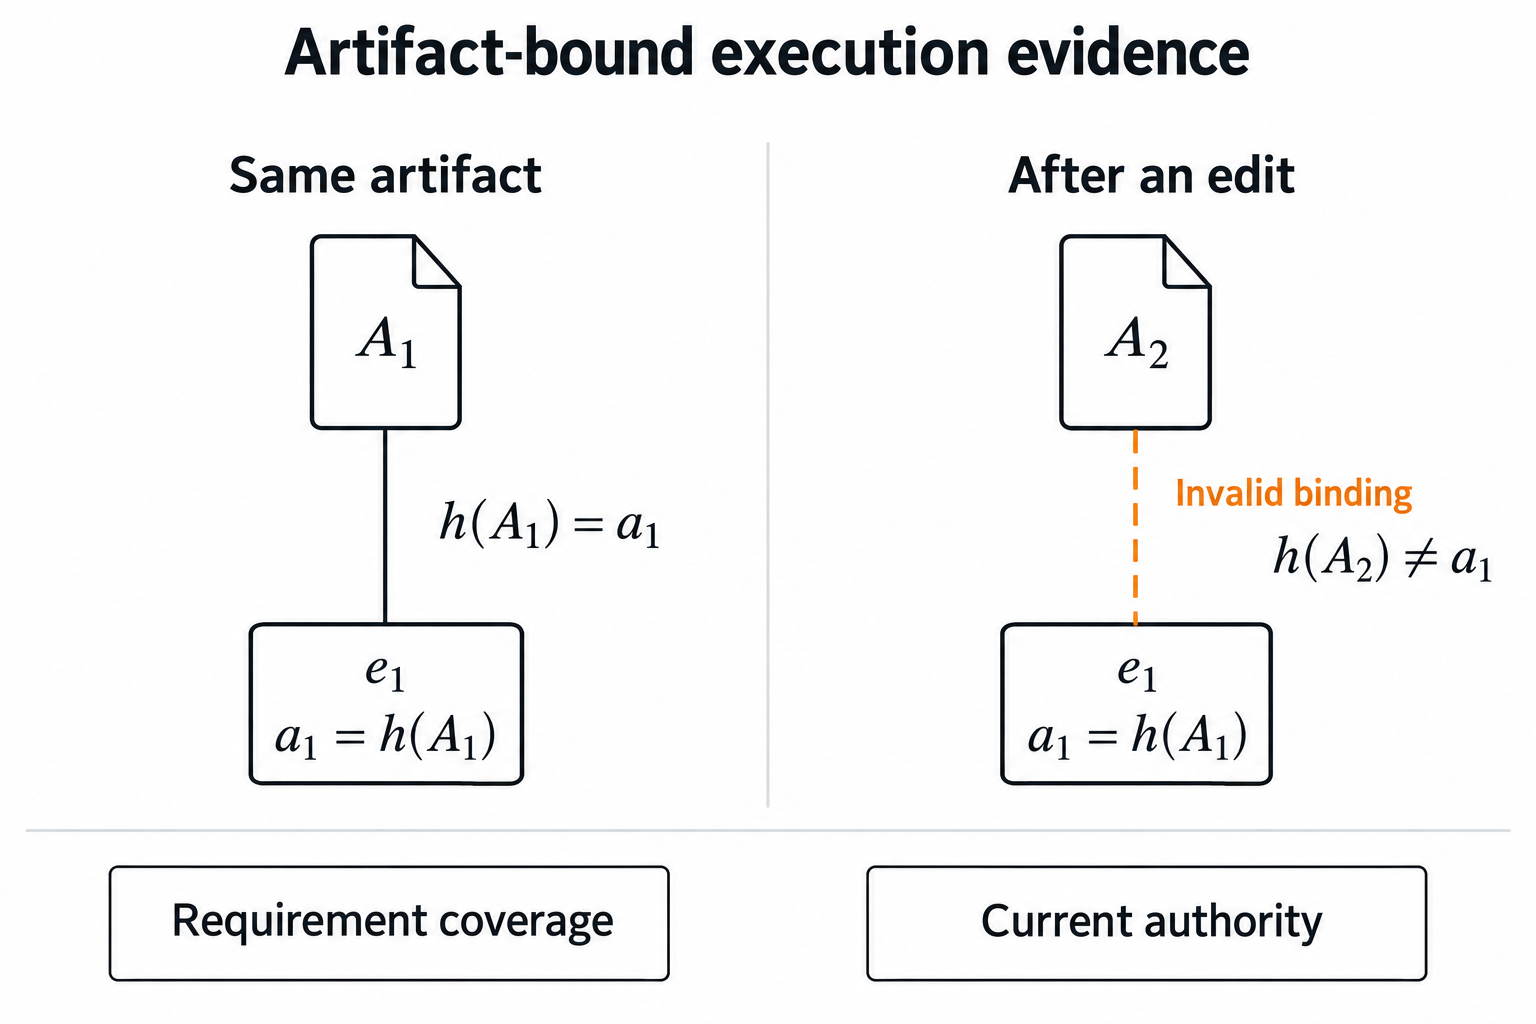
\includegraphics[width=\linewidth]{book/figures/assets/F23review.png}
\caption{The same execution record is checked against two artifact revisions. It binds to the tested artifact in the left panel; the illustrated edit changes the digest and invalidates that binding in the right panel. Matching provenance identifies the object tested, while requirement coverage, the declared environment and current authority need their own checks.}
\label{fig:C23:overview}
\end{figure}

\section{Specifications tests and evaluator blind spots}\label{sec:C23:specification}
Let $\mathcal R$ be the intended requirement set and $\mathcal T$ the executable test set. Passing $\mathcal T$ supports correctness only for the behaviors it covers under the tested environment. It does not imply satisfaction of every element of $\mathcal R$. The gap can arise from missing tests, ambiguous requirements, faulty reference solutions, nondeterministic infrastructure, or a grader that observes the wrong artifact.

A verification gate therefore needs two error rates: false acceptance of a defective artifact and false rejection of a valid artifact. Both depend on the distribution of candidate patches. An evaluator calibrated on ordinary human patches may behave differently on agent-generated solutions that exploit unusual shortcuts. Adaptive optimization against the same visible tests increases this risk because the agent can learn the evaluator's blind spots rather than the task's intended semantics.

For a declared candidate population, let $C\in\{0,1\}$ denote requirement correctness after adjudication and $G\in\{0,1\}$ the grader's acceptance. Write $\pi=P(C=1)$, $s=P(G=1\mid C=1)$, $f=P(G=1\mid C=0)$, and $q=P(G=1)$, assuming both correctness classes have positive probability. The law of total probability gives
\begin{equation}
 q=s\pi+f(1-\pi),\qquad
 \pi=\frac{q-f}{s-f}\quad(s\ne f).
 \label{eq:C23:grader_acceptance_mixture}
\end{equation}
Thus accepted fraction is not identified with correct fraction. If $s=f$, this grader's acceptance carries no information about correctness prevalence in that population. The same decomposition yields $|q-\pi|\leq\max\{f,1-s\}$. These are population identities, not a correction obtained by importing a false-acceptance rate from a different benchmark. Estimation requires an independently adjudicated sample of the same candidate process, with uncertainty propagated jointly through $q,s,f$; a small $|s-f|$ makes inversion unstable. Changing agents, search budgets or visible-test exposure can change both conditional error rates. Stress fixtures establish sensitivity to their seeded defects and need not estimate the natural population rates.

SWE-Bench Pro increases task complexity and uses public, held-out, and commercial repository groups~\cite{corpus250916941}. Its access structure is important evidence about reproducibility: independently auditing public tasks is not equivalent to reproducing results on unavailable proprietary tasks. A contamination-resistant design also does not prove absence of prior exposure. The survey should preserve those distinctions when comparing numbers across benchmark versions and scaffolds.

A concrete failure case is a patch that handles the sample input but fails on a boundary condition implied by the specification. Another modifies a serialization path correctly while breaking a related caller absent from the visible tests. A third passes locally but depends on an undeclared environment variable. These cases require different interventions: requirement-derived tests, integration coverage, and environment capture. More chain-of-thought tokens do not directly repair an evaluator that never checks the failing behavior.

Reference implementations are useful but fallible. A differential test that distinguishes a candidate from a reference detects disagreement; it establishes a defect only if the reference behavior follows the requirement. Human or model interpretation of that requirement can still err. Report the adjudication procedure and unresolved ambiguity rather than treating reference agreement as mathematical truth. Chapter~\ref{ch:C25} develops this verification boundary further.


\section{Terminal trajectories and learned execution policies}\label{sec:C23:terminal}
Terminal agents expose a broad action space through a compact interface. The same shell can inspect files, run tests, modify dependencies, and invoke network tools. This flexibility reduces the number of specialized APIs needed, but it makes semantic validation harder. A syntactically valid command can have effects far beyond the intended task. The sandbox and permission layer must mediate those effects independently of the model's stated intent.

Long terminal trajectories contain more than command examples. They include evidence gathering, hypothesis revision, failed attempts, recovery, and final artifact validation. TerminalHorizon explicitly studies synthesis of task environments that preserve the work needed for these behaviors~\cite{corpus261013166}. Its environment-reconstruction mechanism is relevant because a synthetic setup can accidentally solve the difficult part before the agent begins. A training example then rewards superficial completion rather than the intended exploration.

The current v2 separates a task package into public instruction and environment and private reference solution, verifier and construction configuration. Its independent challenger is uninvolved in construction and solves from the public interface; trace-based diagnosis then guides reconstruction of work accidentally simplified during setup. Progressive expansion adds requirements under the same goal that depend on earlier results and feedback~\cite{corpus261013166}. This is more specific than increasing a maximum turn count. Challenger success alone does not certify absence of every shortcut, and generated verifier agreement remains conditional on its task specification. The appropriate ablation changes reconstruction or expansion separately while preserving model, training tokens and evaluation access, and reports both task coverage and the work demonstrably left for the learner.

The causal comparison should distinguish richer trajectories from easier environments. Keep initial information, required work, and evaluator access comparable across data-generation variants. Audit whether task descriptions leak a solution, whether setup scripts precompute key artifacts, and whether generated tests reveal hidden requirements. Supervised fine-tuning gains on multiple benchmarks can be informative while leaving these construction confounds unresolved.

Trajectory learning also depends on actual behavior conditioning. If a training pipeline reconstructs context after the fact and removes information the policy originally saw, logged actions no longer correspond to the assumed policy inputs. MemoryWalker addresses this class of mismatch~\cite{j2026memorywalker}. For coding agents, record context edits, tool-output truncation, and environment version along with actions. A repository checkout and final patch are insufficient to reconstruct the decision process.

Evaluation should report progress through the full task rather than command validity alone. Measure artifact success, constraints, execution cost, recovery, and whether the final output identifies tested and untested behavior. A terminal agent that produces a plausible explanation after failing to run tests should not receive the same completion status as one with verified results. Conversely, an infrastructure outage should remain visible as an environmental failure rather than be silently removed from the denominator.


The inspected mini-swe-agent release 2.4.6, dated 23 July 2026, explicitly counts billed calls that fail parsing against the cost limit\cite{executionrelease08}. This small implementation detail materially changes budget-matched evaluation: excluding paid malformed responses would give a system additional effective resources while reporting the same nominal limit. It is a concrete example of why a minimal loop remains useful as a research baseline but still requires release-level inspection. The relevant experiment compares identical malformed-output schedules before and after the accounting change, measuring budget overshoot and completed work rather than inferring a reasoning improvement from the release note.

The pinned implementation confirms a further boundary. \path{DefaultAgent.query} checks already accumulated cost before the next model call; successful calls add returned cost, while the \path{FormatError} recovery branch adds reported billed cost from the exception record~\cite{cumb2026minisweloop}. This is post-charge accounting, not the reservation protocol of Chapter~\ref{ch:C20}. For one serial query loop, assume admission and cost updates are serialized, at most one charge remains unrecorded in flight, and each charge is recorded before admitting the next call. If $B>0$ is the active threshold, the initial total is below $B$, and each newly admitted call costs at most $c_{\max}$, the pre-call check bounds the charged total by $B+c_{\max}$, rather than by $B$. Parallel callers can all pass a stale total, so the one-call bound is not a global concurrency guarantee. Without a known call-cost ceiling there is no finite overshoot bound from that check alone. Tool fees and environment charges outside this counter require separate accounting. A reproducible budget comparison must therefore distinguish a declared stopping threshold from a guaranteed maximum expenditure.

\section{Computer use grounding and hidden state}\label{sec:C23:computeruse}
Computer-use agents act through visual observations and input events. The policy must connect screen coordinates or semantic targets to application state, often across scrolling, asynchronous updates, and multiple windows. A click can be delivered successfully to the wrong object. Therefore transport acknowledgment and task correctness are especially far apart. The environment should record both intended target and observed result where the interface permits it.

Coordinate systems require explicit transformations. Let $x_m\in\mathbb R^2$ be a point in the image presented to the model, $p$ its letterbox offset, $w,h>0$ the rendered content dimensions, and $w_c,h_c>0$ the corresponding crop dimensions in physical screenshot pixels. If $c$ is the crop offset inside a screenshot whose desktop origin is $o$, the adapter must apply
\begin{equation}
 x_{\mathrm{desktop}}=o+c+
 \operatorname{diag}(w_c/w,h_c/h)(x_m-p).
\end{equation}
The expression assumes axis-aligned resizing without rotation and one physical-pixel coordinate system; CSS coordinates or device-independent units require an additional declared transform. Points outside the content rectangle should be rejected rather than clamped onto an unintended control. A deterministic mapping defect can dominate performance while being misdiagnosed as poor visual reasoning. Tests should perturb resolution, crop, letterboxing, viewport and display scaling independently. Even a correct map becomes stale if the application moves the target between observation and dispatch, so the observation identity and permitted delay remain part of the action contract.

There is a useful sufficient condition for geometric targeting, with deliberately limited scope. Let $A=\operatorname{diag}(w_c/w,h_c/h)$, suppose the model-space localization error is at most $\epsilon_m$, and bound the remaining calibration residual on the relevant image region by $\epsilon_c$. During delay $\Delta t$, assume the target region undergoes only a rigid translation of norm at most $v\Delta t$. If the intended desktop point has interior margin $r$ to the target's complement at observation time, then
\begin{equation}
 \|A\|_2\epsilon_m+\epsilon_c+v\Delta t<r
 \label{eq:C23:target_margin}
\end{equation}
ensures the dispatched point remains inside the translated target region: the triangle inequality bounds its displacement relative to that region by the left-hand side. This is an analytical interface condition, not an estimated guarantee for a vision model. Reflow, disappearance, occlusion, disabled controls, focus changes and a wrong semantic target invalidate or fall outside the hypotheses. Even an inside-region click still requires outcome verification. The condition explains why timestamped observations, calibration tests and a new screenshot after layout changes can address distinct failure mechanisms.

Screenshots are incomplete observations. They may omit hidden cells, collapsed panels, off-screen recipients, background downloads, or permission dialogs. A final screenshot showing a document title does not establish that the document contains the required data. Agents need application-specific verification or additional observations. When APIs are available, they can provide stronger state evidence, but the evaluation must declare whether the agent or only the evaluator can use them.

AgentHorizon evaluates judges on instruction-trajectory pairs, including closely related instructions whose trajectories are not interchangeable~\cite{corpus261011050}. This paired design exposes a common failure: accepting a trajectory because it looks like successful work while missing a constraint that distinguishes the actual request. The result concerns judge reliability, not merely executor capability. It motivates storing sufficient history for verification while also testing whether a judge can locate the relevant evidence.

An experiment should separate perception, target selection, action delivery, and outcome verification. Oracle target coordinates quantify perception headroom; replayed actions quantify environment determinism; authoritative state checks audit the final judge. The oracle conditions are diagnostic controls, not deployable capabilities. Report how much each stage contributes to failure and how those contributions change with task horizon. A single end-to-end score cannot identify which interface should be improved.


\section{Coding product families and observable tests}\label{sec:C23:catalog}
Table~\ref{tab:C23:catalog} places coding, terminal, editor, and application-building systems into one comparison program without treating them as equivalent. A product may span local and remote execution, and an exposed client does not make its entire service inspectable. The official surfaces were rechecked on 29 October 2026; experimental claims require the corresponding executable configuration and evidence. Retrieval failure on a product homepage is not a capability verdict: Lovable's official documentation establishes its application-building and code-export surfaces, while the resolved Antigravity 2.0 announcement distinguishes a standalone agent application from its separate IDE~\cite{cumb2026lovable,cumb2026antigravity2}.
\begingroup\setlength{\tabcolsep}{3pt}\small
\bookneedspace{.42\textheight}
\begin{longtable}{L{25mm}L{35mm}L{48mm}}
\caption{Coding and computer-work product surfaces and diagnostic tests.}\label{tab:C23:catalog}\\
\toprule Product & Inspected role & Diagnostic condition \\
\midrule\endfirsthead
\toprule Product & Inspected role & Diagnostic condition \\
\midrule\endhead
Codex\cite{executionproduct005} & Open harness and SDK boundaries & Bind final artifacts to tested revisions; separate local execution from hosted service state. \\
OpenHands\cite{executionproduct008} & Self-hosted software-agent workflows & Inspect sandbox reset and replay after environment loss. \\
goose\cite{executionproduct009} & Local extensible tool automation & Audit extension authority and effects outside the workspace. \\
Warp\cite{executionproduct013} & Terminal and cloud development surfaces & Compare local state with remotely delegated job state at interruption. \\
Kilo\cite{executionproduct015} & Multi-model coding interfaces & Hold the selected model fixed before attributing gains to orchestration. \\
OpenCode\cite{executionproduct016} & Extensible coding runtime & Change tool schemas and test stored session compatibility. \\
Letta Code / Letta harness\cite{executionproduct017} & Stateful coding and editable memory & Revoke an old instruction and test its influence on resumed work. \\
Claude Code\cite{executionproduct021} & Terminal coding and developer integration & Verify permission enforcement independently of model-generated intent. \\
GitHub Copilot\cite{executionproduct022} & Repository editor and delegated coding surfaces & Distinguish IDE suggestions from autonomous remote task execution. \\
Cline\cite{executionproduct023} & Configurable local coding automation & Inject a failing command and inspect confirmation and retry behavior. \\
Zed Agent\cite{executionproduct025} & Editor with native and external agents & Test unsaved buffers, external-agent context and artifact identity. \\
Cursor\cite{executionproduct027} & Editor and cloud coding interfaces & Audit which project state reaches background workers and their final merge. \\
Sourcegraph Agentic Batch Changes\cite{executionproduct028} & Batch repository-change workflow & Measure migration coverage and per-repository regressions rather than one patch score. \\
Hermes Agent\cite{executionproduct030} & Persistent agent with memory and skills & Separate stored procedures from learned weight updates and test stale-skill effects. \\
Mistral Vibe\cite{executionproduct036} & Coding CLI and work interfaces & Identify local command mediation and managed conversation boundaries. \\
Devin\cite{executionproduct037} & Delegated engineering environments & Verify reproducible environment setup and independently test the delivered patch. \\
Factory Droids\cite{executionproduct038} & Local and cloud engineering work & Track workspace reuse, credential scope and review artifact provenance. \\
Amp\cite{executionproduct050} & Persistent coding threads & Interrupt work after tool dispatch and inspect repeated effects on resumption. \\
Antigravity\cite{cumb2026antigravity2} & Standalone agent app and separate IDE & Test project-scoped context, subagents and permissions under the selected product surface. \\
Qwen Code\cite{cumb2026qwencode} & Coding runtime with selectable model adapters & Match model and tool serialization before comparing repository results. \\
mini-swe-agent\cite{executionproduct065} & Minimal research coding loop & Use as a low-complexity baseline with identical evaluator and budget. \\
Junie\cite{executionproduct067} & IDE, CLI and delegated coding workflow & Separate test execution evidence from generated explanations of correctness. \\
Harness Cosmos / Auggie\cite{executionproduct069} & Enterprise code-context tooling & Provider lineage does not prove shared implementation; test repository-context boundaries. \\
Kiro\cite{executionproduct070} & Specification-oriented development & Perturb a requirement after planning and test invalidation of dependent work. \\
Rovo Dev\cite{executionproduct073} & Issue-context engineering workflow & Verify that ticket permissions and repository write permissions remain distinct. \\
Replit Agent\cite{executionproduct074} & Application construction and deployment & Validate deployed behavior and environment configuration, not preview appearance alone. \\
MiniMax Code\cite{executionproduct075} & Persistent mini-app and task surfaces & Test background-task lifecycle and whether saved artifacts match verified output. \\
Tabnine Agent / Plugin for OpenCode\cite{executionproduct086,cumb2026tabnineopencode} & Enterprise coding distribution & Verify selected binary, provider lockdown and tool-governance configuration. \\
v0\cite{executionproduct087} & Generated full-stack web applications & Test backend access controls, deployment identity and post-generation regressions. \\
Lovable\cite{cumb2026lovable} & Full-stack app building and code export & Bind preview, exported code and published deployment to the same reviewed artifact. \\
CodeBuddy\cite{executionproduct095} & Subagent interface documentation & Test isolated contexts, inherited permissions and integration of conflicting edits. \\
TRAE / SOLO\cite{executionproduct096} & IDE and standalone task agent & Separate interactive assistance from unattended completion under the same task contract. \\
ZCode\cite{executionproduct097} & Desktop coding with tool interfaces & Audit memory persistence and browser authority separately from coding quality. \\
\bottomrule\end{longtable}
\endgroup


The important mechanisms cut across these families. Editor integration can reduce navigation cost and expose project context, but it can also hide unsaved state or privileged extensions. Cloud delegation can provide isolated environments and parallel work, but adds environment reconstruction and artifact-transfer boundaries. Application builders can integrate deployment tightly, but task success must then include the deployed artifact and its operational configuration rather than only a generated preview.

Codex's documented SDK and open harness interfaces provide concrete inspection boundaries, while its hosted application and services remain separate components~\cite{executionproduct005}. Claude Code's public repository and SDK documentation likewise require artifact-specific interpretation~\cite{executionproduct021,executionproduct020}. No claim of complete implementation visibility follows from a public issue tracker or client repository. For both families, experiments must identify what runs locally, what runs remotely, and where state and authority are enforced.

The current inventory also contains consequential context-lifecycle distinctions. Letta Code's pinned README describes memory, skills, prompts and harness modifications as adaptation surfaces; its cloud backend manages bundled default prompts on resume unless the documented preservation option is selected. That is a configuration transition requiring capture, not evidence of a fixed policy or autonomous weight improvement~\cite{cumb2026lettacode}. Qwen Code exposes multiple provider protocols and SDK/desktop/browser interfaces, so treating every Qwen Code run as one Qwen model is incorrect~\cite{cumb2026qwencode}. Tabnine's OpenCode distribution supplies its own managed binary, Tabnine-served model selection and organization controls; sharing an underlying agent family does not establish equivalence to a separately configured OpenCode installation~\cite{cumb2026tabnineopencode}. Provider lineage and product packaging must remain distinct from the manifest of an evaluated run.

In the pinned Codex TypeScript SDK, \texttt{CodexExec.run} spawns the CLI with a JSON event stream, and \texttt{Thread.run} reduces completed-item events into a buffered return value. A turn-failure event causes that buffered path to throw; completed items accumulated earlier are not returned as a successful \texttt{Turn}. The streaming path exposes events as they arrive~\cite{cumb2026codexsdk}. An application needing partial-progress recovery should durably record relevant events and artifact identities while streaming, rather than infer that a thrown turn produced no work. Neither stream persistence nor a completed-item event by itself certifies the absence of unresolved remote effects. This is a source-level distinction between event delivery and task completion, not an independently measured failure rate.


\section{A budget-matched evaluation protocol}\label{sec:C23:experiments}
The evaluation unit is a task plus initial environment, permitted resources, and scoring contract. Pin repository commit, dependency state, tool versions, model identity where available, and product configuration. If a hosted product does not expose a stable model or harness revision, record the retrieval and execution dates and restrict conclusions to the observed service. A nominally repeated experiment can change when the provider updates an opaque component.

Use task-level paired comparisons. Each system receives the same problem and a reset environment, with task order randomized where persistent memory is enabled. Declare whether memory may transfer between repositories or projects. A system with privileged workspace history has a different information budget from a fresh baseline. This difference may be a legitimate deployment advantage, but it must not be misrepresented as an intrinsic model gain.

Resource accounting includes input and output tokens, tool fees, environment startup, waiting, retries, verifier work, and human intervention. Report elapsed time and monetary cost separately. A cloud product can exploit parallel resources unavailable to a local baseline; matching elapsed time alone then compares different total compute. Conversely, matching dollars may permit different wall-clock and environment availability. The comparison axes should precede any ranking.

Ablations should target interfaces as well as prompts. Compare full repository search with restricted retrieval, executable feedback with model-only critique, persistent workspace with fresh workspace, and independent samples with coordinated subagents. Preserve test access and scoring across conditions. Where a product does not permit a component ablation, report the complete configured treatment rather than inventing an internal causal explanation.

Failure analysis should retain invalid calls, unexecuted tests, timeouts, partial patches, and inaccessible tasks. Distinguish infrastructure failures from policy errors without removing either from overall operational reliability. Confidence intervals should cluster repeated attempts by task and repository where applicable. If the sample is too small to distinguish adjacent products, report that uncertainty rather than converting a noisy ordering into a purchasing recommendation.


\section{Artifact authority and reviewable completion}\label{sec:C23:completion}
A coding agent's final message should identify the artifact, the checks actually executed, their outcomes, and material limitations. This is not merely presentation quality. It gives the recipient the evidence needed to distinguish a proposed solution from a validated change. A confident statement that tests pass is not evidence if the trace records a skipped or failed command. The harness should generate factual execution status from authoritative records whenever possible.

Reviewable completion requires a stable artifact boundary. In version control, that can be a commit digest or patch against a known base. In a browser-created application, it can be an exported bundle and deployment identifier. In a computer-use task, it can be an authoritative application record with its permission state. The boundary varies, but it must allow the verifier to inspect the same object the agent claims to have completed.

Human review is an additional control, not an oracle. Reviewers have limited time, may anchor on the agent's explanation, and may not inspect every dependency or generated file. The agent should therefore expose high-risk changes and missing evidence rather than bury them in a long narrative. Evaluation can measure whether reviewers detect seeded defects under a fixed review budget. It should not claim safety merely because a workflow contains an approval button.

The strongest engineering design binds authority to the transition being approved. Approval of a patch does not authorize later unrelated edits; approval to prepare a deployment does not necessarily authorize publication. If the artifact changes after review, the approval's dependency digest should fail validation. A resumed session must recheck current permissions even if its history contains an earlier grant. These conditions connect coding agents to the broader authorization analysis of Chapter~\ref{ch:C29}.

The practical conclusion is that coding and computer-use competence is a property of an evidence-producing execution system. Better models expand what can be attempted. Better interfaces reduce avoidable friction. Stronger evaluators identify a larger subset of defects. Durable state and authority checks keep long tasks coherent. Each layer has an identifiable contribution and a residual failure surface. Scientific comparison requires preserving those layers rather than attributing every successful artifact to an undifferentiated agent product.

\section{A concrete grading failure and its discriminating controls}\label{sec:C23:gradingcase}
Consider a task requiring a report to be saved in a particular project folder without changing its sharing settings. A computer-use trajectory creates a report with the correct title and visible content, but saves it in a similarly named personal folder. A judge that examines only the final screenshot may accept it. The error is not necessarily poor visual recognition: the relevant distinction may be absent from that screenshot. A stronger model given the same incomplete evidence cannot reliably infer the missing location.

The first control supplies an authoritative folder identifier to the judge while leaving the executor unchanged. If acceptance errors disappear, the observation interface is implicated. The second control provides the full trajectory, including the save dialog, but no authoritative identifier. This tests whether historical evidence is sufficient and whether the judge can retrieve it. The third swaps the instruction for a closely related request that would be satisfied by the observed trajectory. This tests whether the judge checks instruction-specific constraints rather than rewarding generic task plausibility. AgentHorizon's paired instruction design directly motivates this distinction~\cite{corpus261011050}.

An analogous repository failure occurs when an agent changes a public function's return format while preserving the sample command's output. Unit tests focused on the sample pass, but a downstream caller breaks. Supplying more model-generated critique may or may not find the defect. A requirement-derived integration test provides a different kind of evidence because it executes the affected contract. Yet the test can still be wrong if it encodes an interpretation not required by the task. The evaluation must therefore retain both the executable failure and its requirement justification.

Causal diagnosis records the full execution and scoring chain. The task contains a constraint; the executor either overlooks it or lacks an adequate observation; the artifact violates it; the grader fails to inspect the decisive evidence; the final score reports success. Intervening only on the last step corrects the benchmark label but does not improve the executor. Intervening on the executor can improve artifacts while leaving the grader vulnerable to future failure classes. These are separate research contributions and should not share one undifferentiated reliability claim.

The implementation ledger for this case identifies the task adapter, initial state constructor, action executor, trace serializer, grader input builder, and acceptance function. At each boundary, record whether the decisive folder identifier or function contract remains available. A missing field is a concrete engineering finding. A present field ignored by the judge is a model or prompting finding. A correct judge verdict overwritten by a scoring adapter is an evaluation implementation finding. Locating the boundary prevents expensive model changes from being used to compensate for a deterministic data-loss defect.

The proposed experiment reports false acceptance, false rejection, evidence sufficiency, and evaluator cost under each control. Tasks are paired by instruction family, so uncertainty must preserve that pairing. Seeded defects help establish diagnostic sensitivity but do not estimate their natural deployment prevalence. Real trajectory audits complement them by identifying failures the fixture designer did not anticipate. The combination supplies a stronger basis for improvement than either a large leaderboard score or a handful of impressive demonstrations.

Deployment also requires a distributional statement. Folder-confusion fixtures test sensitivity to deliberately ambiguous names rather than overall product quality. A low frequency in a small natural sample does not exclude the failure. Combine stress-test sensitivity with an uncertain estimate of deployment exposure. When an error changes permissions or publishes an artifact, its tail consequence can dominate despite high average completion.

